\section{Vision Controle}\insertloftspace
\setcounter{figure}{0}\setcounter{table}{0}

The joystick was an explicit request from our client that he wanted us to implement. However, he wanted to relocate the workforce from the United States to Asian countries such as the Philippines. We, therefore, warned him about possible problems, especially the latency time for such a system. Indeed, the distance between Manila (the capital of the Philippines) and Los Angeles is 11,759 km. Assuming that we have a cable connecting them, which is very unlikely, the information can travel at the speed of light. A command will therefore take $\displaystyle{\frac{11759}{3.10^5}=0.04s}$. The duration between the sending of a command and the video return would be 0.08s which is considerable and would make the operation very complicated.

\bigbreak
We then looked for solutions that did not involve artificial intelligence to address this problem. However, since we still had to develop a solution using a joystick, we ran out of time. It is nevertheless a promising solution. To implement these solutions, we used the python openCV library\cite{opencvPython}. We trained ourself thanks to a python book and youtube channels.

\subsection{3D position}

Our first one consisted in making the user select the desired tomato and then estimating its 3D position using a camera. We kept the user without the need to send the order live. 

\bigbreak
The depth cameras being relatively expensive, we decided to buy only a stereo camera and to build a software able to determine the depth. All this process is done in the camera frame. It is a camera with two lenses that can retrieve two synchronized images.

\bigbreak
Using the youtube channel and the GitHub page of \textit{Nicolai Nielsen}, we calibrated the lenses to standardize the images received. Once this was done, we were able to calculate the \gls{disparity}\footnote{The apparent motion of objects between a pair of stereo images}. OpenCv has a class that allows to perform such a calcul for a calibrated \gls{sc}\footnote{A camera with two or more lenses with a separate image sensor or film frame for each lens}. Some parameters needed to be tune, and we did it thanks to sidebar until we considered we obtained the best disparity image. The code can be found on appendix \ref{disparityCode}.
\begin{figure}[H]
    \begin{subfigure}{.5\linewidth}
        \centering
        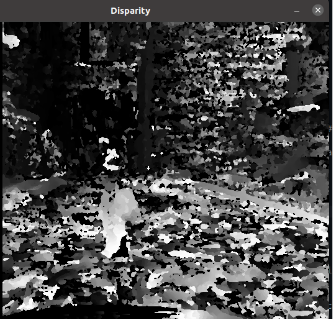
\includegraphics[width=0.8\textwidth]{Images/Section08/disparity.png}
        \caption{Disparity}
        \label{fig:disparity}
    \end{subfigure}%
    \begin{subfigure}{.5\linewidth}
        \centering
        \includegraphics[width=1\textwidth]{Images/Section08/stereo\_camera\_view.png}
        \caption{Camera view}
        \label{fig:Stereoview}
    \end{subfigure}\\[1ex]
    \caption{Stereo camera image}
    \label{fig:Sci}
\end{figure}
\FloatBarrier

The figure below shows an image and its disparity. You can see that the tomato stands out a little, in a white mass. We can also note that the farther the elements on the image are, the darker they appear on the disparity image. There is indeed a correlation between disparity and distance. These are inversely proportional. To find the coefficient, we then took photos of an object at different distances known then we calculated the disparity. We then obtain the curves below which give the relationship between depth and disparity.
\begin{figure}[H]
    \centering
    \includegraphics[width=0.8\textwidth]{Images/Section08/depth\_disparity.png}
    \caption{Disparity depth relation}
    \label{fig:DisparityDepth}
\end{figure}
\FloatBarrier

Similarly, there is a link between depth and size of a pixel. Indeed, the closer an image will be, the more it will take a large place in the image. Once we were able to obtain the distance along the z axis, we wanted to calculate the position in x,y. We then sought the relationship in depth and size of a pixel. We have measured the size in pixel of the same object of known size for different depths and then we have drawn the curve. A polynomial of degree 3 seems to stick to the curve on the desired interval (10-40cm).
\begin{figure}[H]
    \centering
    \includegraphics[width=0.6\textwidth]{Images/Section08/depth\_pixel\_size.png}
    \caption{Depth pixel size relation}
    \label{fig:DepthPixel}
\end{figure}
\FloatBarrier

The center of the image corresponds to the position (0,0). The user clicks on the center of the tomato, to get the central pixel. Using the first relation we are able to provide the distance to the camera. Then we calculate the pixel distance between the center and this point and with the second relation we calculate the position in m. We then obtain the 3D position of the center of the tomato.  We then calculate the position in the base frame and the inverse kinematics as shown in the diagram below.
\begin{figure}[H]
    \centering
    \includegraphics[width=0.8\textwidth]{Images/Section08/position\_schema.png}
    \caption{3D position schema}
    \label{fig:PositionSchema}
\end{figure}
\FloatBarrier

\bigbreak
Unfortunately, our solution was not precise enough. Setting up the disparity calculation with openCV would have required more time and for the same tomato, we could vary by several centimeters.

\subsection{Tracking}

The second idea consisted in object tracking. As in the previous solution, the user selects the tomato and a software developed with openCV allows to track it.
\begin{figure}[H]
    \begin{subfigure}{\linewidth}
        \centering
        \includegraphics[width=0.4\textwidth]{Images/Section08/tracking\_view.png}
        \caption{Camera view}
        \label{fig:View}
    \end{subfigure}\\[1ex]
    \begin{subfigure}{.5\linewidth}
        \centering
        \includegraphics[width=0.8\textwidth]{Images/Section08/tracking\_no\_filter.png}
        \caption{no tracking}
        \label{fig:notracking}
    \end{subfigure}%
    \begin{subfigure}{.5\linewidth}
        \centering
        \includegraphics[width=0.8\textwidth]{Images/Section08/tracking\_filter.png}
        \caption{tracking}
        \label{fig:tracking}
    \end{subfigure}\\[1ex]
    \caption{Computer tracking view}
    \label{fig:trackingView}
\end{figure}
\FloatBarrier

Once the tomato has been selected, a filter is applied to our image: only elements similar to the one chosen are kept. We can see that the chair in front of the camera disappears when the tracking is activated. Visually, a square highlighting the selected tomato appears on the image too.

\bigbreak
To transform this into a command, the green dot on the image in the center of the met corresponds to the lens. We must therefore center the tomato on this point. To do this, we calculate the distance in pixels between the two and we apply a command proportional to this distance on the xy plane in the camera frame. Once the tomato is centered, we can move the arm to the tomato. The overall operation is summarized in the diagram below.

\begin{figure}[H]
    \centering
    \includegraphics[width=0.8\textwidth]{Images/Section08/tracking\_schema.png}
    \caption{Object tracking schema}
    \label{fig:TrackingSchema}
\end{figure}
\FloatBarrier

Two problems then arose for us. First, our tracking system was still relatively sensitive and the arm had to move slowly at the risk of losing the tracking. Finally, we had not yet solved the question of how to stop the arm once it moves forward centered on the tomato. 